% !TeX root = ../Project2.tex
\section{Methods}
\label{sec:methods}
\subsection{The Data: Regression}
In this project, the input data is normally distributed, and consist of 100 data points.
The target data is generated by Runge's function, with added noise,
Runge Function which is a one-dimensional function of second order.
\[
  f(x) = \frac{1}{1 + 25x^2}
\]
The noise is normally distributed with a mean of 0 and a 
standard deviation of $0.1$.  
\subsubsection{Reshaping the data}
The input and output data are reshaped into column vectors, (100,1),
this is useful since most machine learning tools expect input features
as a 2D array. \cite{Codex} 
For linear regression problems, the input data is expressed
in terms of polynomial features, which is done
by creating the design matrix of variable degree with the input data x,
and adjusting the features during training, this is equal for ordinary least squares, lasso and ridge. 
For the neural network this is not necessary, since the network architecture,
the number of nodes and layers, replaces the polynomial features, and the 
weights and biases are adjusted during training.  
% Scaling?
\subsection{The algorithm}
The set-up.
\begin{enumerate}
    \item Fix the architecture: the number of inputs and outputs,
    the number of hidden layers and the number of nodes in each.
    \item Choose activation functions for the hidden layers and for the
    output layer, the latter dictated by the range of the target.
    \item Choose the cost function, again dictated by the distribution of the target,
    and any regularisation terms with their hyperparameters
    \item Choose the optimiser - plain gradient dsecent, RMSprop, adam -
    and its learning rate.
    \item Initialise the weights and biases
\end{enumerate}

\begin{figure}[!htbp]
    \centering
    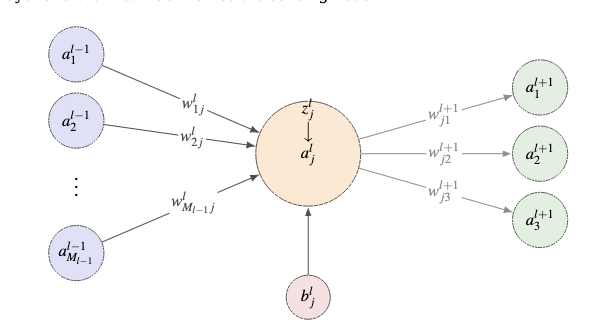
\includegraphics[width=\linewidth]{Figures/Fig8_6.png}
    \caption{The index convention for the equations below, seen from a single node $a_j^{(l)}$. The node $j$ in layer $l$ collects the outputs $a_i^{(l-1)}$ of all $M_{l-1}$ nodes in the previous layer, weighted by $w_{ij}^{(l)}$, adds its own bias $b_j^{(l)}$ to form the pre-activation $z_j^{(l)}$, and applies its activation function $\sigma$ to obtain $a_j^{(l)}$, which it then sends on to every node of layer $l+1$ through the weights $w_{jk}^{(l+1)}$.}
    \label{fig:Indexconvention}
\end{figure}

For a single node, the pre-activation and activation are
\[
    z_j^{(l)} = \sum_{i=1}^{M_{l-1}} w_{ij}^{(l)} a_i^{(l-1)} + b_j^{(l)},
\]
\[
    a_j^{(l)} = \sigma\!\left(z_j^{(l)}\right).
\]
\cite[p.~326--328]{LectureNotes}

Each iteration:
\begin{enumerate}
    \item \textit{Forward pass}. Set $a^{(0)} = x$ and compute $z^{(l)}$ and
    $a^{(l)} = \sigma(z^{(l)})$ for $l = 1, 2, \ldots, L$, storing every
    $z^{(l)}$ and $a^{(l)}$:
    \[
        z^{(l)} = a^{(l-1)} W^{(l)} + b^{(l)},
        \qquad
        a^{(l)} = \sigma\!\left(z^{(l)}\right).
    \]
    \item \textit{Output error}. For a differentiable output activation, compute
    \[
        \delta^{(L)}
        = \sigma'\!\left(z^{(L)}\right)
          \odot \frac{\partial C}{\partial a^{(L)}}.
    \]
    For softmax with cross-entropy, use
    \[
        \delta^{(L)} = \frac{a^{(L)} - y}{n}.
    \]
    \item \textit{Backward pass}. For $l = L-1, L-2, \ldots, 1$, compute
    \[
        \delta^{(l)}
        = \left(\delta^{(l+1)} (W^{(l+1)})^\top\right)
          \odot \sigma'\!\left(z^{(l)}\right).
    \]
    \item \textit{Gradients}. Form
    $\frac{\partial C}{\partial W^{(l)}} =
    (a^{(l-1)})^\top \delta^{(l)}$ and
    $\frac{\partial C}{\partial b^{(l)}} =
    \sum_{i=1}^{n} \delta_i^{(l)}$.
    \item \textit{Update}. With stochastic gradient descent and learning rate
    $\gamma$, update the weights and biases:
    \[
        W^{(l)} \leftarrow W^{(l)}
            - \gamma (a^{(l-1)})^\top \delta^{(l)},
        \qquad
        b^{(l)} \leftarrow b^{(l)}
            - \gamma \sum_{i=1}^{n} \delta_i^{(l)}.
    \]
\end{enumerate}
\cite[p.~350]{LectureNotes}
%LLM Declaration: Copilot GPT Luna 6.0: Fix bugs and syntax errors in enumerate and equations
\subsubsection{Backpropagation}
The backpropagation is the most important part of the neural network,
as it is this process that creates the gradients of each layer, which are used
to update the weights and biases. This process is different depending
on the cost function, since the derivative of the cost function 
is the value we want to minimize. Thus it is different for the
regression problem, which uses mean squared error, and the classification
which uses cross entropy. 
The input layers, the z values and the output values a is generated
by the feed forward pass saver, the backpropagation iterates backwards,
from the last layer to the first. 
% LLM Declaration: Edit skeleton
Regressor, mean squared error:
\begin{align}
    \text{Output layer:}\quad
    \frac{\partial C}{\partial a^{(L)}}
    &= \text{cost function derivative}, \\[4pt]
    \text{Hidden layer:}\quad
    \frac{\partial C}{\partial a^{(l)}}
    &= \delta^{(l+1)} \left(W^{(l+1)}\right)^\top, \\[4pt]
    \delta^{(l)}
    = \frac{\partial C}{\partial z^{(l)}}
    &= \frac{\partial C}{\partial a^{(l)}} \odot
       \sigma'\!\left(z^{(l)}\right), \\[4pt]
    \frac{\partial C}{\partial W^{(l)}}
    &= \left(a^{(l-1)}\right)^\top \delta^{(l)}, \\[4pt]
    \frac{\partial C}{\partial b^{(l)}}
    &= \sum_{i=1}^{n} \delta_i^{(l)}, \\[4pt]
    \nabla^{(l)}
    &= \left(
       \frac{\partial C}{\partial W^{(l)}},
       \frac{\partial C}{\partial b^{(l)}}
       \right).
\end{align}
Cross entropy, classification. 
% LLM structural correction
\begin{align}
    \text{Output layer:}\quad
    \Delta^{(L)}
    &= \frac{\partial C}{\partial Z^{(L)}}
     = \frac{A^{(L)} - Y}{n}, \\[4pt]
    \text{Hidden layers:}\quad
    &
    \begin{aligned}
        \Delta^{(l)}
        &= \frac{\partial C}{\partial Z^{(l)}} \\
        &= \left(\Delta^{(l+1)} (W^{(l+1)})^\top\right) \\
        &\qquad \odot \sigma'\!\left(Z^{(l)}\right), \\
        &\qquad l = L-1,\ldots,1.
    \end{aligned}
\end{align}
\subsection{Stochastic Gradient Descent}
The stochastic gradient descent function trains the neural network over a specified 
number of epochs. One epoch is one pass through the training data. 
At the start of each epoch, the data are shuffled and divided into mini-batches, 
each containing up to \texttt{batch\_size} examples. 
Thus, for \(N\) training examples and batch size \(B\), each epoch contains 
\(\lceil N/B\rceil\) mini-batches. 
The network is updated after each mini-batch, using gradients calculated 
from that batch with backpropagfation. 
This is called mini-batch stochastic gradient descent.
In the implementation, the backpropagation alghorithm calculates the mini-batch gradients, 
and the selected optimizer, plain, adam or rmsprop, updates the weights and biases.
L1 or L2 penalty terms can also be added to the weight gradients, corresponding to Lasso and Ridge. 
The optimizer is selected separately from the mini-batch training procedure.
% LLM Declaration, some text generated with ChatGPT-Sol 6.1
\subsection{Neuralnetregressor}
This estimator wraps the network in a scikit-learn-compatible interface. Its
\texttt{fit} method creates the network using the requested input size and
hidden-layer architecture. It selects the hidden activation function and its
derivative, uses the identity function at the output layer, and supplies the
mean squared error cost and its derivative.

Training is delegated to \texttt{train\_sgd} or \texttt{train\_plain},
according to the \texttt{descent} parameter. For SGD, the \texttt{method}
parameter selects plain gradient descent, Adam, or RMSprop. The training
function updates the weights and biases; the fitted network and training
history are retained by the regressor.

The \texttt{predict} method passes new inputs through the fitted network and
returns a one-dimensional NumPy array with one continuous prediction per
example.
% LLM Generated text: Copilot GPT Luna 6.0
\subsection{Implementation and analysis of Regressor}
\subsubsection{Model verification}
The neuralnetregressor is implemented as an object, and verified against manually 
creating a neural network object and using stochastic gradient descent
to train the model, both objects predict on the same data and the 
mean squared error are calculated on the same data, to ensure they agree. 
The gradients calculated by the backpropagation algorithm, 
are valified by calculating the gradient on the same data by
automatic differentiation using jax. Jax is a verified solution
used by scientists and data analysists, thus this verification ensures
that the backpropagation calculates the correct gradients.
\paragraph{Gradient and training validation}
We tested a network with one hidden layer of 50 nodes and a network with two
hidden layers of 50 and 100 nodes. Both used sigmoid hidden-layer
activations. For all three training methods, the manually calculated
gradients matched those from \texttt{jax.grad} according to
\texttt{np.allclose}. The regressor and manual SGD implementations also
produced matching predictions.

\begin{table}[htbp]
    \centering
    \caption{Gradient validation and training MSE for a network with one
    hidden layer of 50 nodes.}
    \label{tab:regressor-val}
    \begin{tabular}{lccc}
        \hline
        Method & Gradient val. & Regressor val. & SGD train MSE\\
        \hline
        Plain   & Passed & Passed & 0.1031 \\
        Adam    & Passed & Passed & 0.02404  \\
        RMSprop & Passed & Passed & 0.02142  \\
        \hline
    \end{tabular}
\end{table}
\begin{table}[htbp]
    \centering
    \caption{Gradient validation and SGD training MSE for a network with
    two hidden layers containing 50 and 100 nodes, respectively.}
    \label{tab:regressor-val-two-layers}
    \begin{tabular}{lccc}
        \hline
        Method & Gradient val. & Regressor val. & SGD train MSE \\
        \hline
        Plain   & Passed & Passed & 0.1084  \\
        Adam    & Passed & Passed & 0.01873 \\
        RMSprop & Passed & Passed & 0.01394 \\
        \hline
    \end{tabular}
\end{table}
The gradient validation passed for all methods, and both the regressor and the
manual use of sgd agreed. Adam and RMSprop achieved lower training 
MSE than plain stochastic gradient descent. The code can be found at
\cite{FYSSTK4155Prosjekt2ProsjektKode}
% Link to code?

\subsection{Model selection}
\subsubsection{Skicit Learn}
Scikit-learn has multiple classes that can be used to validate and
select between different models. The following classes have been utilised
in the analysis of the Neuralnetwork regressor, 
\begin{enumerate}
    \item $\mathbf{KFold}$: Creates k folds with shuffled values, k is set to 5 in this project. With random state = 2026.
    \item $\mathbf{make_pipeline}$: Creates a pipeline with scikit`s StandardScaler() from the training data, with the NeuralNetRegressor as a chosen model.
    \item $\mathbf{cross_val_score}$: Splits the input data and target values, using the Kfold splitter, fits the pipeline on the training portion of each split, and evaluates it on the validation set of the split. Returns one score per split, with standard deviation.
    \item $\mathbf{cross_validate}$: Does the same operation as cross val score, returns the training score in addition to the validation score for each fold, with standard deviation. Both classes should return the same validation score.
    \item $\mathbf{GridSearchCV}$: The GridSearchCV is the most extensively used class in this project. It uses the same Kfold class and pipeline as the previous cross validation classes. 
    It has an additional $parameter_grid$ input, which uses the input values of the neuralnetregressor as variable model parameters, this allows for models selection on different parameters, such as 
    the learning rate, number of hidden layers and gradient descent methods, plain, adam and rmsprop. This class creates and stores models for all chosen parameters within the grid, and fits on the chosen data using the regressor, and returns the cross validation scores on the training and validation set, the chosen score for the regressor is the negative mean squared error.
\end{enumerate}
\subsubsection{Cross Validation}
The first $\mathbf{make_pipeline}$ is created with the NeuralNetRegressor class with
one hidden layer of 50 nodes, sigmoid as activaiton function of the hidden layer,
a learning rate of $0.01$ with plain gradient descent as the standard method, 
the epoch is set to $100$ with stochastic gradient descent with a batch size of $10$. 
The seed is set to $2026$. 
$\mathbf{KFold}$ is set with 5 folds, shuffle and random state with seed $2026$.
Both cross validation methods on this particular regressor model, is chosen with negative mean squared error
as the scoring value. 
\subsubsection{GridSearchCV}
The gridsearch cross validation is done using the chosen Kfold and neural network regression class
as input variables. The cross validation is done with a different parameter
grid and GridSearchCV model for each step, after each step the best model parameters within one standard error
of the mean squared error is chosen, and used in the next neural regressor model, which in turn is 
the chosen model for the new GridSearchCV model.  
GridSearchCV stores the best model and its scorer, the best model corresponds to the lowest validation mean squared error of all the models.
The first parameter grid is. 
\begin{table}[htbp]
    \centering
    \caption{Parameter grid 1}
    \label{tab:ParamGrid1}
    \begin{tabular}{lccccc}
        \hline
        Parameter & \multicolumn{5}{c}{Values}\\
        \hline
        Gamma  & 0.001 & 0.003 & 0.01 & 0.03 & 0.01\\
        Method & rmsprop & adam & plain \\
        Hidden & (50,) & (50, 100)\\
        \hline
    \end{tabular}
\end{table}[htbp]
Best model parameters within ONE-SE is found through analysing the results of the GridSearchCV,
the best model parameters gamma $- learning rate$, method and hidden layers are chosen for the next
neuralnetregressor model input of the next GridSearch. The second parameter grid is.  
\begin{table}[htbp]
    \centering
    \caption{Parameter grid 2}
    \label{tab:ParamGrid2}
    \begin{tabular}{lccccc}
        \hline
        Parameter & \multicolumn{4}{c}{Values}\\
        \hline
        Activation  & sigmoid & relu\\
        Hidden & (50,) & (30,) & (50, 100,) &(50, 100, 100,)\\
        \hline
    \end{tabular}
\end{table}[htbp]
\begin{table}[htbp]
    \centering
    \caption{Parameter grid 3}
    \label{tab:ParamGrid3}
    \begin{tabular}{lccccc}
        \hline
        Parameter & \multicolumn{4}{c}{Values}\\
        \hline
        Penalty  & None   & L1    & L2 \\
        Lambda   & 0.0001 & 0.001 & 0.01 & 0.1 \\
        Gamma    & 0.003  & 0.01  & 0.03 & 0.1 \\
        \hline
    \end{tabular}
\end{table}[htbp]
Here lambda equals the value of the penalty, L1 and L2 are the norms. 
The last parameter grid is split in half, where lambda is set to zero 
when the penalty is None, else the lambda values are as shown in the table.
\paragraph{One SE}
It is important to specify what is meant by a one se model in this project. 
When a model is chosen during cross validation, based on the lowest mean squared
error, if another model has a mse is within one standard error of the lowest, 
the choice between these two models would be arbitrary if mse was the only qualification,
since one cannot tell, which model actually has the lowest mse, because the standard
error reaches around both models mse. Thus, between these two models 
the least complex, most efficient model is chosen, this is also true
if more than two models are within one se of the best. What model to choose then
within one se of the best model, is then dependent on the model and the
parameters which are varied during the cross validation.
\subsubsection{Linear Regression}
The first \hyperref[tab:ParamGrid1]{parameter grid} is compared 
with linear regression, imported from skicit learn, the pipeline includes
$StandardScaler()$ and $PolynomialFeatures()$. The pipeline is 
cross validated over polynomial degrees $(1,16)$ using GridSearchCV. 
\subsubsection{Dissapearing gradient}
The second parameter grid explore if there is signs of 
dissapearing gradients using the sigmoid activation function, as opposed
to the relu function, with a varied network layer depth and width.
\subsubsection{Lasso and Ridge}
The second parameter grid, which explores widderent penalty norms and values,
along with learning rate during the cross validation search. The results are 
then compared with Lasso and Ridge of degrees $(1, 16)$ and different 
penalty values, $\alpha$, using Sci-kit Linear model classes, pipeline and GridSearchCV. 
The Ridge linear model uses singular valua decompostion "svd" as its solver, while 
Lasso has a max iteration count of $100000$.
\subsubsection{Final test}
The best model from the OLS comparison is tested on data generated by a different
$seed = 1$, the same is done for the Lasso and Ridge comparison. The data is 
predicted on the test data and the mean squared error is calculated between
the predicted values and the target test values. 

\subsection{Neuralnetclassifier}
The \texttt{NeuralNetClassifier} class provides a scikit-learn-compatible
interface for training the project's neural network on classification tasks.
During \texttt{fit}, it records the unique class labels and converts the
training targets to one-hot vectors. The network has one output node per class,
with softmax producing a probability distribution over the classes. Hidden
layers use the selected activation function, and training minimises the
cross-entropy loss.

The class delegates mini-batch training to \texttt{train\_sgd}. Its parameters
specify the hidden-layer sizes and activation, learning rate, optimiser,
regularisation, number of epochs, batch size, and random seed. The
\texttt{predict\_proba} method returns the predicted class probabilities,
while \texttt{predict} selects the class with the highest probability and maps
it back to its original label. Its \texttt{accuracy} method evaluates predicted
labels against the targets. This interface lets the classifier be used with
scikit-learn tools such as pipelines and cross-validation.  
The activation function of the output layer is the softmax, and the cost function
is the cross entropy, as mentioned earlier.
% LLM Declaration: Generated with Copilot using GPT Luna 6.0
\subsubsection{The data}
The data used in the classification problem is the multiclass MNIST data set of handritten digits,
see the description of the data set at https://www.tensorflow.org/datasets/catalog/mnist. 
The data set comes with a canonical split into 60 000 training images and 10 000 test images, 
each a $28 x 28$ array of grey scale pixel values between 0 and 255. 
The training data is separated randomly into two smalles subsets with 1000 data points each, 
as shown in the code section below:
\begin{figure}[htbp]
    \centering
    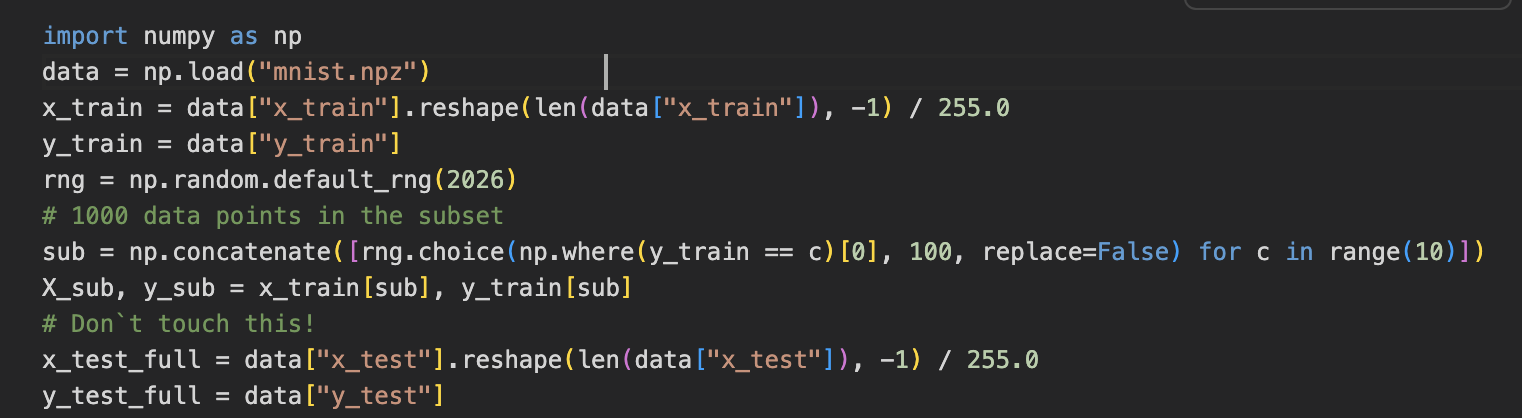
\includegraphics[width=\linewidth]{Figures/MNIST.png}
    \caption{The canonical split of the data set and the subset of the training data, flattening and scaling of input data}
    \label{fig:MNIST}
\end{figure}
The network takes a vector as input, so the image is flattened to a vector of 784 features and scaled
to the interval $[0,1]$. \cite{Project2} The full test data is kept aside for the last test, so that no
data leaks into the training.
\subsubsection{GridSearchCV}
The pipeline for the classification problem is established with Scikit-learns NeuralNetClassifier
with 100 epochs and a batch size of 50, with 1000 data points this corresponds to 20 mini batches per epoch.
The Kfold is created using 5 folds with random state 2026, using the Scikit class StratifiedKFold, a variation
of the KFold that returns stratified folds, the folds are made by preserving the percentage of samples
for each class in the target data in a multiclass classification setting. \cite{StratifiedKFold}
The parameter grid is created in two parts, with a common grid consisting of parameter values:
$$hidden = [(32, ), (64, ), (128,), (64,128,)]$$
$$gamma = [0.001, 0.01, 0.03, 0.1]$$
$$method = ["plain", "adam", "rmsprop"]$$
$$activation = ["relu", "simoid"]$$
The full parameter grid consist of the common grid without Penalty and with L1 and L2 Penalty
with penalty values:
$$lambda = [0.0001, 0.001, 0.01]$$
The Gridsearch is created with these parameter values, the Stratified Kfold, the NeuralNetClassification class
with standard values and scoring = "accuracy". 
\subsubsection{Measure of quality}
\subsubsection{Confusion matrix}